\section{Feature scaling}

\begin{frame}{Why scale features?}
    \begin{columns}[T]
        \begin{column}{0.62\textwidth}
                        \begin{itemize}
                \item Many methods combine features through distances, dot products or a shared penalty
                \item Then units decide a feature's influence: height in centimeters has 100 times the spread of height in meters, though both carry the same information
                \item In USArrests (lecture 10), Assault has an SD of 83.3 and Murder only 4.4
                \item On the raw scale, Assault accounts for 95.6\% of the total variance; after standardizing, every variable accounts for 25\%
            \end{itemize}
        \end{column}
        \begin{column}{0.36\textwidth}
            \centering
            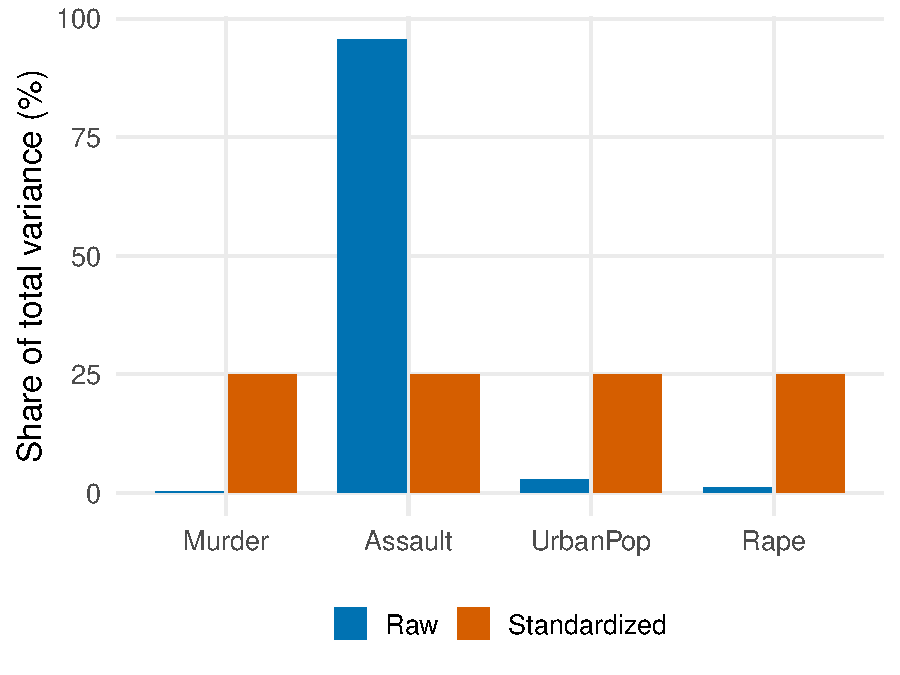
\includegraphics[width=\textwidth, height=0.75\textheight, keepaspectratio]{figures/fig_usarrests_variance.pdf}

            {\scriptsize USArrests: share of total variance}
        \end{column}
    \end{columns}
\end{frame}

\begin{frame}{Three common scalers}
    For feature $j$ with values $x_j^{(1)}, \dots, x_j^{(n)}$:
    \begin{itemize}
        \item Standardization ($z$-score): $\displaystyle z_j^{(i)} = \frac{x_j^{(i)} - \bar{x}_j}{s_j}$, mean $0$ and SD $1$
        \item Min-max scaling: $\displaystyle \frac{x_j^{(i)} - \min_l x_j^{(l)}}{\max_l x_j^{(l)} - \min_l x_j^{(l)}}$, range exactly $[0, 1]$
        \item Robust scaling: $\displaystyle \frac{x_j^{(i)} - \operatorname{median}_j}{\operatorname{IQR}_j}$, median $0$ and IQR $1$
    \end{itemize}
    \svspace{0.3em}
    \centering
    \footnotesize
    \begin{tabular}{@{}l l l l@{}}
        \toprule
        Scaler & Center & Spread & Affected by outliers \\
        \midrule
        Standardization & mean & standard deviation & yes \\
        Min-max & minimum & range & strongly \\
        Robust & median & IQR (width of the middle half) & hardly \\
        \bottomrule
    \end{tabular}
\end{frame}

\begin{frame}{A small example}
    \centering
    \begin{tabular}{@{}l r r r r r@{}}
        \toprule
        $x$ & 2 & 4 & 6 & 8 & 30 \\
        \midrule
        Standardized ($\bar{x} = 10$, $s = 11.4$) & $-0.70$ & $-0.53$ & $-0.35$ & $-0.18$ & $1.75$ \\
        Min-max ($\min = 2$, $\max = 30$) & $0.00$ & $0.07$ & $0.14$ & $0.21$ & $1.00$ \\
        Robust (median $6$, IQR $4$) & $-1.0$ & $-0.5$ & $0.0$ & $0.5$ & $6.0$ \\
        \bottomrule
    \end{tabular}

    \svspace{0.8em}
    \raggedright
    \begin{itemize}
        \item The value 30 pulls the mean up and inflates the SD, so the other four standardized values bunch together below 0
        \item Min-max squeezes the four regular values into $[0, 0.21]$
        \item Robust scaling keeps their spacing ($0.5$ apart) and leaves 30 clearly visible as an outlier at $6$
    \end{itemize}
\end{frame}

\begin{frame}{Normalization: two meanings}
    \begin{columns}[T]
        \begin{column}{0.56\textwidth}
                        \begin{itemize}
                \item ``Normalization'' can mean min-max scaling of a feature (a column), or rescaling each observation (a row) to unit length:
                \[
                    \mathbf{x}^{(i)} \mapsto \frac{\mathbf{x}^{(i)}}{\lVert \mathbf{x}^{(i)} \rVert}
                \]
                \item Each row keeps its direction but loses its length, so dot products become cosine similarities
                \item Common for word counts, so that long documents do not dominate
            \end{itemize}
        \end{column}
        \begin{column}{0.42\textwidth}
            \centering
            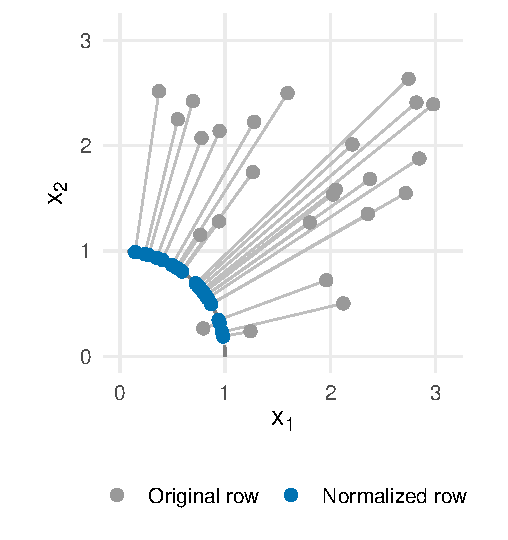
\includegraphics[width=\textwidth, height=0.65\textheight, keepaspectratio]{figures/fig_unit_norm.pdf}

            {\scriptsize 25 rows with lengths from 0.84 to 3.82, each rescaled to length 1}
        \end{column}
    \end{columns}
\end{frame}

\begin{frame}{Scalers: details}
    \begin{itemize}
        \item All three scalers are linear maps $x \mapsto (x - a)/b$, fitted separately for each feature: they shift and stretch a feature but never change the shape of its distribution
        \item pandas' \texttt{std()} divides by $n - 1$ (the sample SD), scikit-learn's \texttt{StandardScaler} by the SD with denominator $n$; the difference only matters for tiny samples
        \item In this course, ``scaling'' always means a per-feature transformation; row normalization is named explicitly whenever it is used
        \item In scikit-learn the two are \texttt{MinMaxScaler} (columns) and \texttt{Normalizer} (rows)
    \end{itemize}
\end{frame}

\begin{frame}{Which models need scaling?}
    \centering
    \footnotesize
    \begin{tabular}{@{}l c l@{}}
        \toprule
        Model & Scale? & Why \\
        \midrule
        $k$-NN, clustering & yes & distances sum differences over features \\
        SVM with RBF kernel & yes & the kernel is a function of distances \\
        PCA (lecture 12) & yes & directions of largest variance \\
        Ridge, lasso, elastic net & yes & one penalty shared by all coefficients \\
        Neural nets, gradient descent & yes & convergence depends on the loss shape \\
        OLS, logistic (no penalty) & no & predictions unchanged \\
        Trees, random forests, boosting & no & splits use only the order of values \\
        \bottomrule
    \end{tabular}

    \medskip
    {\scriptsize SVM: support vector machine. RBF: radial basis function. A kernel is a similarity score between two observations: high for similar points, close to 0 for very different ones}
\end{frame}

\begin{frame}{Reading the table}
    \begin{itemize}
        \item Rule of thumb: scaling matters when one number (a distance, a penalty, a step size) is shared across features, so a feature's unit decides its influence; it does not matter when the method can absorb a change of unit, as OLS does by rescaling its coefficient, or uses only the order of values, as trees do
        \item ``No'' in the last two rows refers to the predictions
        \item Scaling still changes how the coefficients of a linear model read: a standardized coefficient is the change in the response for a one-SD change in the feature
        \item scikit-learn's \texttt{LogisticRegression} adds an $L_2$ penalty by default, so in practice it belongs to the ``yes'' group unless the penalty is switched off
    \end{itemize}
\end{frame}

% \begin{frame}{Kernel: a similarity score}
    % \begin{columns}[T]
        % \begin{column}{0.62\textwidth}
            % \begin{itemize}
                % \item A kernel $K(\mathbf{x}, \mathbf{x}')$ turns two observations into one number: how alike they are
                % \item Identical customers get the maximum, customers with little in common get close to 0
                % \item The RBF kernel rates similarity by distance: $K = \exp(-\gamma \lVert \mathbf{x} - \mathbf{x}' \rVert^2)$ is 1 at distance 0 and fades toward 0 as the distance grows
                % \item Large $\gamma$: only very close points are similar; small $\gamma$: similarity reaches far
            % \end{itemize}
        % \end{column}
        % \begin{column}{0.36\textwidth}
            % \centering
            % \begin{tikzpicture}[x=0.85cm, y=2cm, font=\scriptsize]
                % \draw[->] (0, 0) -- (4.3, 0) node[below left] {distance};
                % \draw[->] (0, 0) -- (0, 1.2) node[above] {similarity};
                % \draw (0.05, 1) -- (-0.05, 1) node[left] {1};
                % \node[left] at (0, 0) {0};
                % \draw[thick, blue!70!black, domain=0:4.2, samples=60, smooth] plot (\x, {exp(-0.15*\x*\x)});
                % \draw[thick, orange!90!black, domain=0:4.2, samples=60, smooth] plot (\x, {exp(-1.5*\x*\x)});
                % \node[blue!70!black, anchor=west] at (2.4, 0.58) {small $\gamma$};
                % \node[orange!90!black, anchor=west] at (1.05, 0.3) {large $\gamma$};
            % \end{tikzpicture}
        % \end{column}
    % \end{columns}
% \end{frame}

\begin{frame}{Evidence: Default data}
    \begin{columns}[T]
        \begin{column}{0.52\textwidth}
            \begin{itemize}
                \item We use all 333 defaults and 333 random non-defaults
                \item In 50 random 70/30 splits, balance (SD 602) and income (SD 13{,}616) are standardized with the training mean and SD
                \item $k$-NN improves from 0.774 to 0.875
                \item The SVM jumps from 0.475, no better than guessing, to 0.877
                \item Logistic regression, the tree and the forest make identical predictions in all 50 splits
            \end{itemize}
        \end{column}
        \begin{column}{0.46\textwidth}
            \centering
            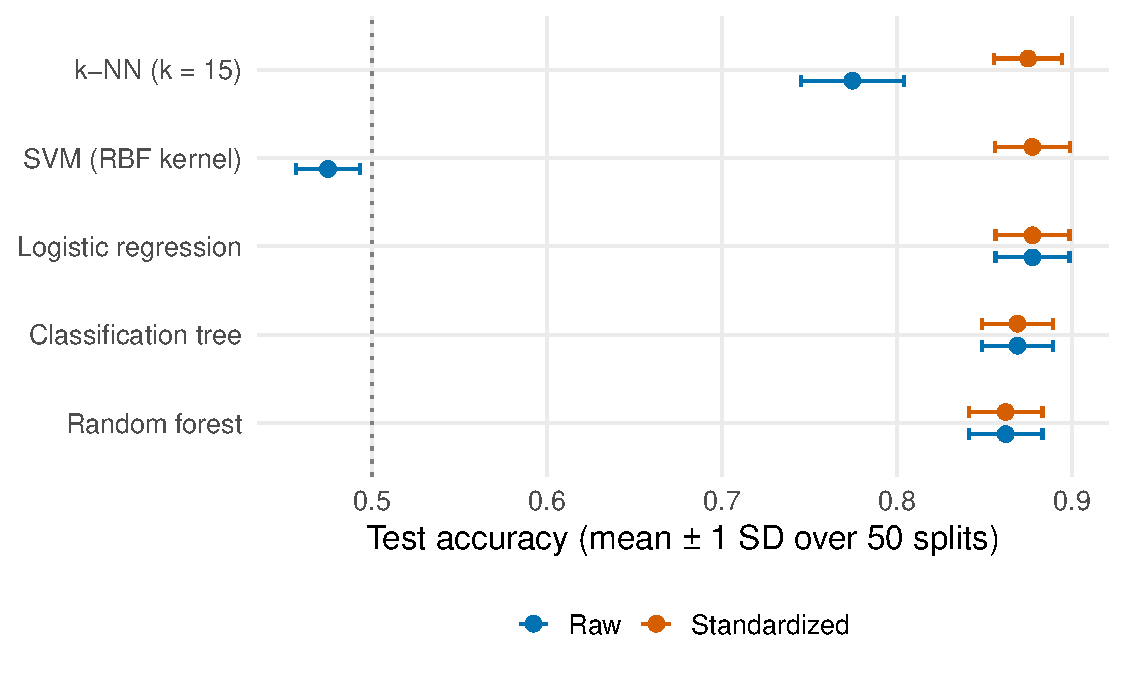
\includegraphics[width=\textwidth, height=0.75\textheight, keepaspectratio]{figures/fig_scaling_models.pdf}

            {\scriptsize Mean test accuracy over 50 splits; dotted line at 0.5}
        \end{column}
    \end{columns}
\end{frame}

\begin{frame}{Behind the Default results}
    \begin{itemize}
        \item Why a balanced subsample: in the full data, 96.7\% of customers do not default, so always answering ``no default'' would already be right 96.7\% of the time
        \item $k$-NN uses $k = 15$: a customer gets the majority label of the 15 most similar customers
        \item The SVM uses the RBF kernel with $\gamma = 1/p$ and cost $C = 1$. Like $k$-NN, it sees the data only through distances, so scaling should affect it in the same way
        \item On the raw data, income differences of thousands of dollars dominate every distance: $k$-NN effectively ignores balance, the feature that predicts default, and for the SVM every pair of different customers gets a similarity of essentially 0
    \end{itemize}
\end{frame}

\begin{frame}{Gradient descent: walking downhill}
    \begin{columns}[T]
        \begin{column}{0.64\textwidth}
            \begin{itemize}
                \item Fitting a model means finding the coefficients with the lowest loss: picture the loss as a landscape, with the best fit at the bottom
                \item Gradient descent is a hiker in fog who feels the slope underfoot, steps downhill, and repeats
                \item Too big a step overshoots the bottom and bounces; too small a step takes forever
                \item Scaling does not change the fitted model, but it reshapes the landscape, and with it the number of steps
            \end{itemize}
        \end{column}
        \begin{column}{0.34\textwidth}
            \centering
            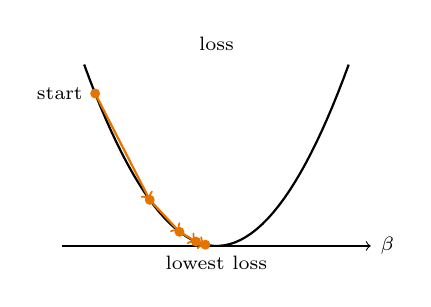
\begin{tikzpicture}[x=0.7cm, y=0.4cm, font=\scriptsize]
                \draw[->] (-2.8, 0) -- (2.8, 0) node[right] {$\beta$};
                \draw[thick, domain=-2.4:2.4, samples=50] plot (\x, {\x*\x});
                \foreach \a/\b in {-2.2/-1.21, -1.21/-0.67, -0.67/-0.37, -0.37/-0.2} {
                    \draw[->, thick, orange!90!black] (\a, {\a*\a}) -- (\b, {\b*\b});
                }
                \foreach \a in {-2.2, -1.21, -0.67, -0.37, -0.2} {
                    \fill[orange!90!black] (\a, {\a*\a}) circle (1.8pt);
                }
                \node[left] at (-2.25, 4.84) {start};
                \node[below] at (0, 0) {lowest loss};
                \node[above] at (0, 5.9) {loss};
            \end{tikzpicture}
        \end{column}
    \end{columns}
\end{frame}

\begin{frame}{Gradient descent and the shape of the loss}
    \centering
    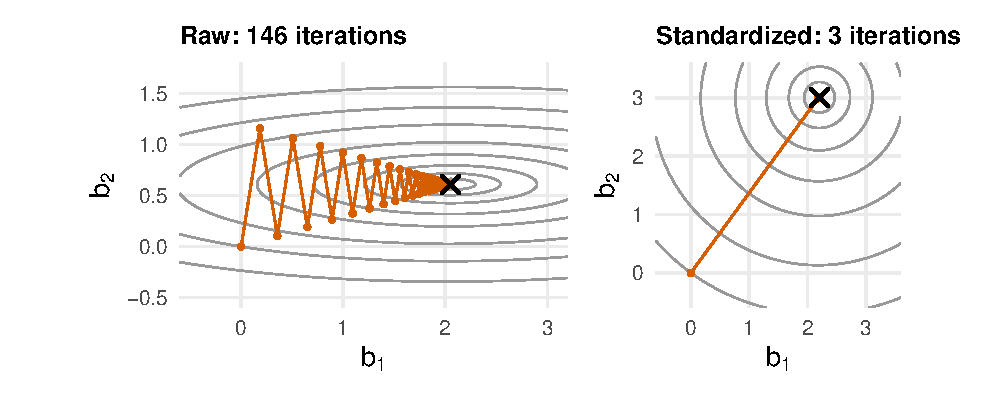
\includegraphics[width=\textwidth, height=0.5\textheight, keepaspectratio]{figures/fig_scaling_contours.pdf}

    {\scriptsize Two simulated features (SD 1.07 and 4.93); gray: loss contours, $\times$: minimum, orange: steps}
    \raggedright
    \begin{itemize}
        \item On raw features the valley is long and narrow: even the best fixed step size needs 146 iterations to reach relative error $10^{-6}$
        \item After standardizing it is a round bowl, and 3 iterations are enough
    \end{itemize}
\end{frame}

\begin{frame}{Why unscaled features stretch the valley}
    \begin{itemize}
        \item A feature with a large spread makes the loss react strongly to its coefficient: moving the coefficient of $x_2$ (SD 4.93) costs far more than moving that of $x_1$ (SD 1.07)
        \item So the landscape is steep along one coefficient and flat along the other; the curvature (how sharply the loss rises away from the best value) is here roughly the variance of the feature
        \item A step small enough not to overshoot on the steep side is too small for quick progress on the flat side, so the path zig-zags across the valley instead of heading for the bottom
        \item The ratio of the steepest to the flattest curvature measures the stretch: 21.1 for the raw features, 1.02 after standardizing (1 is a round bowl). Its technical name is the condition number
    \end{itemize}
\end{frame}

\begin{frame}{Penalized regression: ridge and lasso}
    \begin{itemize}
        \item In linear regression, a penalty can be added to the loss function: a new term containing $\boldsymbol{\beta}$, so that minimizing the loss also shrinks the coefficients
        \item Ridge adds the sum of the squared coefficients and the lasso the sum of their absolute values, each multiplied by a number $\lambda \ge 0$ that sets the strength
        \item Ridge shrinks all coefficients toward 0; the lasso also shrinks them and can set some exactly to 0
        \item Both put one shared price on all coefficients, which is why the units of the features matter here
        \item Ridge and lasso are discussed in detail in the feature selection section
    \end{itemize}
\end{frame}

\begin{frame}{Penalties are not scale-invariant}
    \begin{columns}[T]
        \begin{column}{0.6\textwidth}
                        \begin{itemize}
                \item The ridge penalty $\frac{\lambda}{2} \sum_j \beta_j^2$ treats every coefficient the same, whatever its unit
                \item Credit: Balance on Income and three standardized predictors; only Income's unit changes
                \item Income's OLS coefficient is 0.0063 per dollar, 6.27 per \$1000 and 221 per SD
                \item A small coefficient is barely charged: Income's halves only at $\lambda \approx 1.1 \times 10^{9}$, $1.1 \times 10^{3}$ and $0.95$. Standardize first
            \end{itemize}
        \end{column}
        \begin{column}{0.38\textwidth}
            \centering
            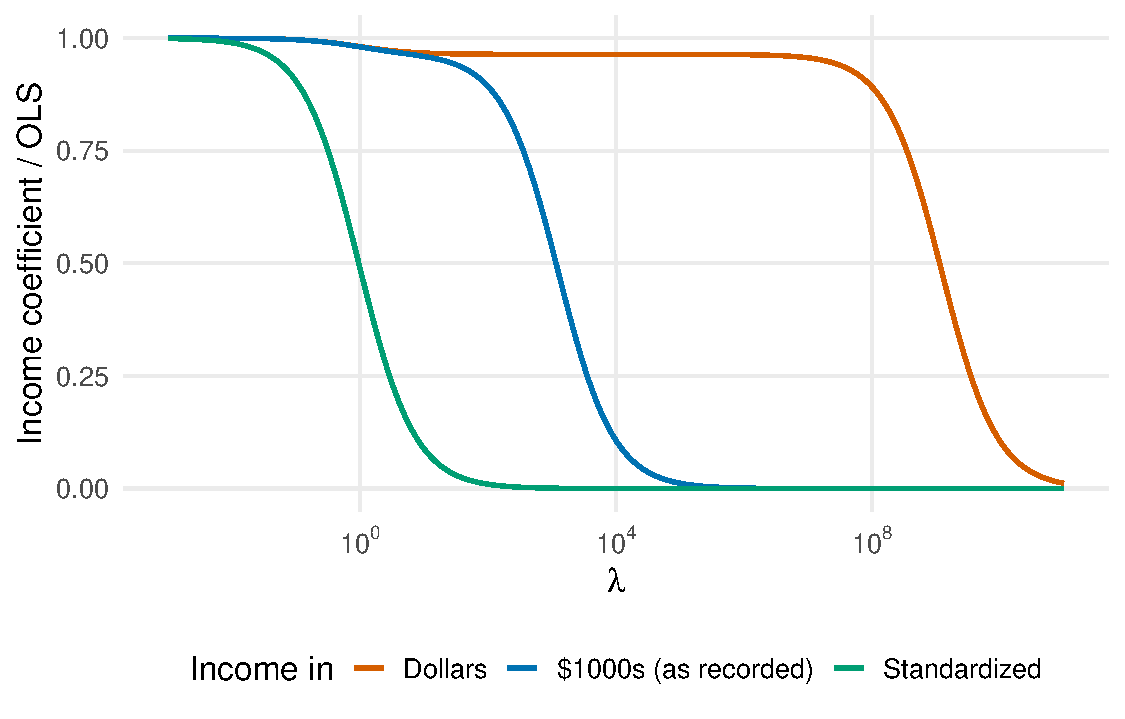
\includegraphics[width=\textwidth, height=0.75\textheight, keepaspectratio]{figures/fig_ridge_units.pdf}
        \end{column}
    \end{columns}
\end{frame}

\begin{frame}{Penalties: details}
    \begin{itemize}
        \item The three predictors next to Income (Age, Cards, Education) are almost uncorrelated with it ($r = 0.18$, $-0.02$ and $-0.03$), so Income's coefficient shrinks because of its own penalty
        \item The $\lambda$ at which it halves is close to the variance of Income in each unit: $1.24 \times 10^9$ in dollars squared, $1{,}242$ in thousands, $1$ standardized
        \item scikit-learn's \texttt{Ridge} and \texttt{Lasso} do not standardize the predictors, so put a \texttt{StandardScaler} in front of them
    \end{itemize}
\end{frame}

\begin{frame}{Outliers and the choice of scaler}
    \begin{columns}[T]
        \begin{column}{0.5\textwidth}
            \begin{itemize}
                \item Each scaler is fitted to 50 regular values, with and without one outlier
                \item Under min-max, the outlier squeezes the regular values from $[0, 1]$ into $[0, 0.17]$
                \item Standardizing shrinks them from $[-2.21, 1.81]$ to $[-0.83, 0.44]$
                \item Robust scaling barely moves them ($[-1.49, 1.31]$); the outlier lands at 15.0, easy to spot
                \item It does not remove the outlier, though
            \end{itemize}
        \end{column}
        \begin{column}{0.48\textwidth}
            \centering
            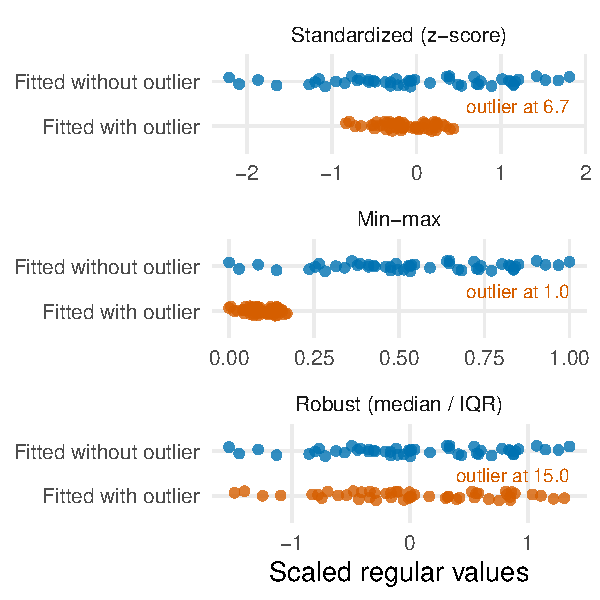
\includegraphics[width=\textwidth, height=0.75\textheight, keepaspectratio]{figures/fig_scalers_outlier.pdf}
        \end{column}
    \end{columns}
\end{frame}

\begin{frame}{Which scaler when? Examples}
    \centering
    \footnotesize
    \renewcommand{\arraystretch}{1.15}
    \begin{tabular}{@{}p{0.17\textwidth} p{0.35\textwidth} p{0.42\textwidth}@{}}
        \toprule
        Scaler & Use it when & Typical features \tabularnewline
        \midrule
        Standardization & \raggedright the feature is roughly symmetric with no extreme values; the default choice & \raggedright a patient's height, weight or blood pressure; exam scores; daily temperature \tabularnewline
        Min-max & \raggedright the feature has natural, known bounds, or the model expects inputs in $[0, 1]$ & \raggedright pixel intensities 0--255 for a neural net; ratings on a 1--5 scale; percentages \tabularnewline
        Robust & \raggedright a few values sit far from the rest and you want to keep them & \raggedright household income; house prices; payment amounts in fraud detection \tabularnewline
        \bottomrule
    \end{tabular}

    \svspace{0.6em}
    \raggedright
    \normalsize
    \begin{itemize}
        \item Ask what the extremes look like. Bounded and fixed: min-max. Unbounded but well behaved: standardize. A long tail or rare extremes: robust (or a log first)
    \end{itemize}
\end{frame}

\begin{frame}{Choosing a scaler in practice}
    \begin{itemize}
        \item When unsure, standardize; if a box plot shows a few points far outside the whiskers, switch to robust scaling
        \item Min-max is safe when the measurement fixes the bounds (a pixel is always 0--255). Fitted on sample extremes, it breaks when a new house costs more than any in the training data: its scaled value exceeds 1
        \item Robust scaling keeps outliers far out instead of squashing the rest; in fraud detection an unusually large payment should stay unusual
        \item Income and prices often do better logged first, then standardized: robust scaling alone keeps the long tail
        \item A \texttt{ColumnTransformer} can scale columns differently: robust for income, min-max for ratings, standardization for age
    \end{itemize}
\end{frame}

\begin{frame}{Skewed features}
    \centering
    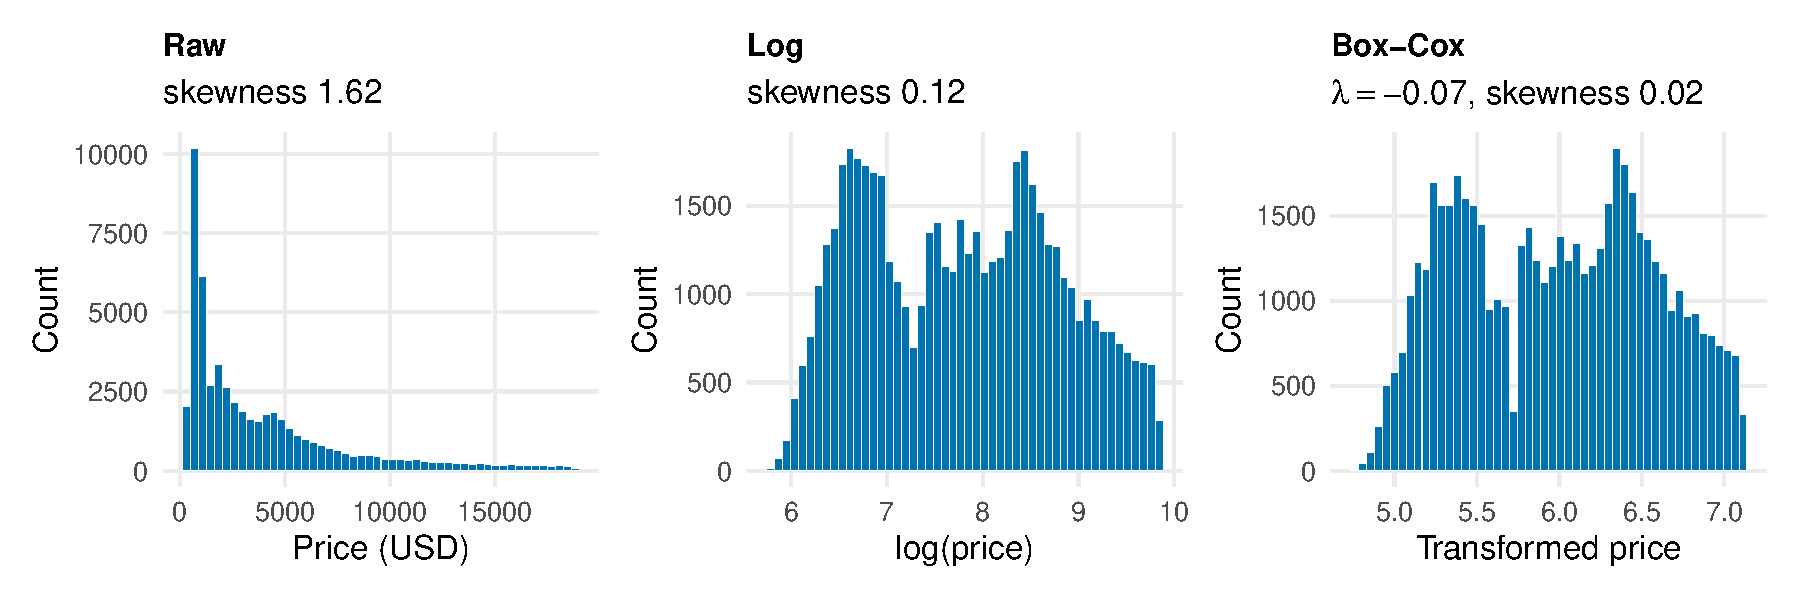
\includegraphics[width=\textwidth, height=0.4\textheight, keepaspectratio]{figures/fig_skew_transforms.pdf}

    {\scriptsize Price of 53{,}940 diamonds (the \texttt{diamonds} data from R's \texttt{ggplot2} package)}
    \raggedright
    \begin{itemize}
        \item Scaling is linear and keeps the shape: skewness is 1.62 before and after standardizing
        \item Taking $\log x$ of a positive, right-skewed feature brings the skewness down to 0.12
        \item Box-Cox, $(x^\lambda - 1)/\lambda$, picks $\lambda$ by maximum likelihood; $\lambda = -0.07$ is close to the log, and the skewness drops to 0.02
    \end{itemize}
\end{frame}

\begin{frame}{Box-Cox and the log}
    \begin{itemize}
        \item The log compresses large values more than small ones, which pulls in a long right tail
        \item Box-Cox picks $\lambda$ by maximum likelihood: in effect, the power that makes the data look most like a bell curve
        \item Box-Cox defines its $\lambda = 0$ member as $\log x$, which is the limit of $(x^\lambda - 1)/\lambda$ as $\lambda \to 0$
        \item Transforming a skewed feature helps models that are sensitive to large values, such as linear models and distance-based methods
        \item Trees are unaffected by any increasing transformation
        \item Yeo-Johnson extends Box-Cox to zero and negative values. Transform first, then scale
    \end{itemize}
\end{frame}

\begin{frame}{Fit the scaler on the training data only}
    \begin{columns}[T]
        \begin{column}{0.5\textwidth}
            \begin{itemize}
                \item A scaler has parameters (mean and SD, min and max, median and IQR) estimated from data
                \item Estimate them on the training data, then apply the same transformation to test data and to new observations
                \item Scaling before the split lets the test data influence the training data, which is called leakage
                \item And at prediction time, a single new observation has no mean or SD of its own to use
            \end{itemize}
        \end{column}
        \begin{column}{0.48\textwidth}
            \centering
            \begin{tikzpicture}[
                    box/.style={draw, rounded corners, minimum width=2.4cm, minimum height=0.75cm, align=center, font=\footnotesize},
                    >={Stealth[length=2mm]}
                ]
                \node[box, fill=blue!10] (train) {Training data};
                \node[box, fill=orange!15, right=0.5cm of train] (test) {Test data};
                \node[box, below=0.7cm of train] (fit) {Fit scaler:\\ $\bar{x}_j$, $s_j$};
                \node[box, fill=blue!10, below=0.7cm of fit] (strain) {Scaled\\ training data};
                \node[box, fill=orange!15, below=2.15cm of test] (stest) {Scaled\\ test data};
                \draw[->] (train) -- (fit);
                \draw[->] (fit) -- (strain);
                \draw[->] (test) -- (stest);
                \draw[->, dashed] (fit.east) -| node[pos=0.25, above, font=\scriptsize] {same $\bar{x}_j$, $s_j$} ([xshift=-0.6cm]stest.north);
            \end{tikzpicture}
        \end{column}
    \end{columns}
\end{frame}

\begin{frame}{Pipelines and cross-validation}
    \begin{columns}[T]
        \begin{column}{0.5\textwidth}
            \begin{itemize}
                \item In $K$-fold CV the held-out fold plays the test set, so every preprocessing step is refitted in each split
                \item A pipeline chains the steps and refits all of them whenever the model is fitted
                \item In scikit-learn, build it with \texttt{make\_pipeline} and pass it to \texttt{cross\_val\_score}; \texttt{ColumnTransformer} handles different columns differently
            \end{itemize}
        \end{column}
        \begin{column}{0.48\textwidth}
            \centering
            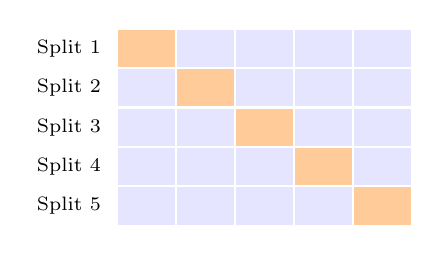
\begin{tikzpicture}[x=0.75cm, y=0.5cm]
                \foreach \r in {1,...,5} {
                    \node[font=\scriptsize, anchor=east] at (0.4, -\r + 0.5) {Split \r};
                    \foreach \c in {1,...,5} {
                        \ifnum\r=\c
                            \fill[orange!40] (\c - 0.5, -\r) rectangle (\c + 0.5, -\r + 1);
                        \else
                            \fill[blue!10] (\c - 0.5, -\r) rectangle (\c + 0.5, -\r + 1);
                        \fi
                        \draw[white, thick] (\c - 0.5, -\r) rectangle (\c + 0.5, -\r + 1);
                    }
                }
            \end{tikzpicture}

            \svspace{0.3em}
            {\scriptsize Fit the scaler, any feature selection and the model on the blue folds; evaluate on the orange fold}
        \end{column}
    \end{columns}
\end{frame}

\begin{frame}{Leakage in practice}
    \begin{itemize}
        \item For scaling the leak is usually small, because a mean and an SD estimated with or without the test rows are nearly the same
        \item The same rule applies to every step that learns from data; for feature selection, which picks features by looking at the labels, the leak can be large
        \item For example, \texttt{cross\_val\_score(make\_pipeline(StandardScaler(), KNeighborsClassifier()), X, y, cv=5)} refits the scaler on the four training folds of each split before fitting $k$-NN
    \end{itemize}
\end{frame}

\begin{frame}{Binary and categorical features}
    \begin{itemize}
        \item 0/1 dummies (indicator variables) are usually left as they are: the unit ``has the category or not'' is already interpretable
        \item In the Default example the student dummy stayed 0/1 in both versions
        \item With ridge or lasso, a dummy's coefficient is penalized like any other; standardizing a dummy divides it by $\sqrt{\hat{p}(1 - \hat{p})}$, which changes how strongly rare categories are penalized
        \item A \texttt{StandardScaler} applied to all columns standardizes the dummies too; whichever choice you make, make it on purpose and apply it the same way in training and prediction
        \item Ordinal codes ($1, 2, 3, \dots$) can be scaled like numeric features if the spacing is meaningful
    \end{itemize}
\end{frame}

\begin{frame}{Scaling: summary}
    \begin{itemize}
        \item Scale features before distance-based methods, kernels, PCA, penalized models and gradient descent; trees and unpenalized linear models do not need it
        \item Standardize by default, use robust scaling when there are outliers, and min-max when you need a bounded range
        \item Transform skewed features (log, Box-Cox, Yeo-Johnson) before scaling
        \item Fit every preprocessing step on training data only, inside a pipeline
    \end{itemize}
\end{frame}


\section{The curse of dimensionality}

\begin{frame}{More features are not free}
    \begin{itemize}
        \item $k$-NN predicts whether a customer defaults from the customers most similar to them
        \item That works when similar customers exist and really are close
        \item Each feature we add makes both harder, even if the number of observations $n$ stays the same
        \item Richard Bellman called this the curse of dimensionality
        \item The next slides build the intuition with uniform data, where everything can be worked out, and then show what it does to real models
    \end{itemize}
\end{frame}

\begin{frame}{The data spread thin}
    \centering
    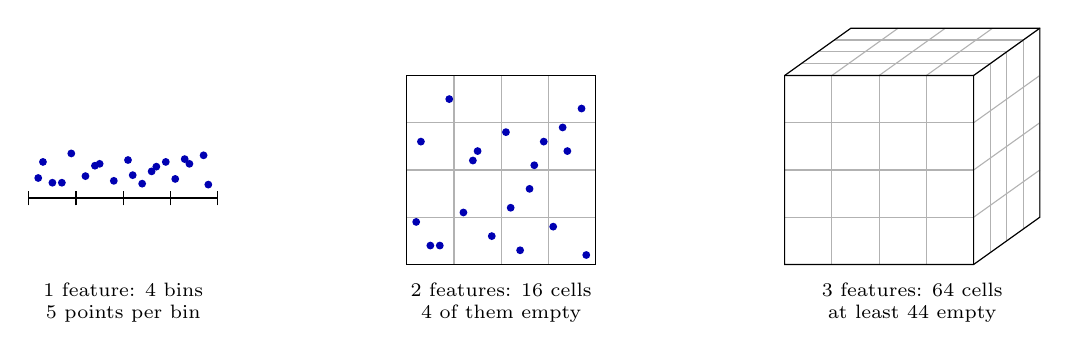
\begin{tikzpicture}[x=0.6cm, y=0.6cm, dot/.style={circle, fill=blue!70!black, inner sep=1pt}]
        % one feature
        \begin{scope}
            \draw[thick] (0, 1.4) -- (4, 1.4);
            \foreach \i in {0, ..., 4} \draw (\i, 1.25) -- (\i, 1.55);
            \foreach \x/\y in {0.3/2.6, 0.7/0.4, 0.9/3.5, 1.2/1.1, 1.5/2.4, 1.8/0.6, 1.4/2.2, 0.5/0.4, 2.1/2.8, 2.4/0.3, 2.6/1.6, 2.9/2.6, 2.2/1.2, 3.1/0.8, 3.4/2.4, 3.7/3.3, 3.3/2.9, 3.8/0.2, 2.7/2.1, 0.2/0.9} \node[dot] at (\x, 1.65 + 0.2 * \y) {};
            \node[font=\scriptsize, align=center] at (2, -0.8) {1 feature: 4 bins\\5 points per bin};
        \end{scope}
        % two features
        \begin{scope}[xshift=4.8cm]
            \draw[step=1, gray!60] (0, 0) grid (4, 4);
            \draw (0, 0) rectangle (4, 4);
            \foreach \x/\y in {0.3/2.6, 0.7/0.4, 0.9/3.5, 1.2/1.1, 1.5/2.4, 1.8/0.6, 1.4/2.2, 0.5/0.4, 2.1/2.8, 2.4/0.3, 2.6/1.6, 2.9/2.6, 2.2/1.2, 3.1/0.8, 3.4/2.4, 3.7/3.3, 3.3/2.9, 3.8/0.2, 2.7/2.1, 0.2/0.9} \node[dot] at (\x, \y) {};
            \node[font=\scriptsize, align=center] at (2, -0.8) {2 features: 16 cells\\4 of them empty};
        \end{scope}
        % three features
        \begin{scope}[xshift=9.6cm]
            \foreach \i in {0, ..., 4} {
                \draw[gray!60] (\i, 0) -- (\i, 4);
                \draw[gray!60] (0, \i) -- (4, \i);
                \draw[gray!60] (\i, 4) -- (\i + 1.4, 5);
                \draw[gray!60] (0.35 * \i, 4 + 0.25 * \i) -- (4 + 0.35 * \i, 4 + 0.25 * \i);
                \draw[gray!60] (4, \i) -- (5.4, \i + 1);
                \draw[gray!60] (4 + 0.35 * \i, 0.25 * \i) -- (4 + 0.35 * \i, 4 + 0.25 * \i);
            }
            \draw (0, 0) -- (4, 0) -- (5.4, 1) -- (5.4, 5) -- (1.4, 5) -- (0, 4) -- cycle;
            \draw (0, 4) -- (4, 4) -- (4, 0) (4, 4) -- (5.4, 5);
            \node[font=\scriptsize, align=center] at (2.7, -0.8) {3 features: 64 cells\\at least 44 empty};
        \end{scope}
    \end{tikzpicture}
    \raggedright
    \begin{itemize}
        \item The same 20 points give 5 per bin with one feature, 1.25 per cell with two and 0.31 with three
        \item Each feature multiplies the cells by 4: with 10 features there are 1{,}048{,}576, and 5 points per cell would take 5{,}242{,}880 points
        \item The data needed grow exponentially with $p$
    \end{itemize}
\end{frame}

\begin{frame}{Neighborhoods stop being local}
    \begin{columns}[T]
        \begin{column}{0.56\textwidth}
            \begin{itemize}
                \item Say $k$-NN uses the 10\% of the data most similar to the new point
                \item With uniform data, how much of each feature's range must that neighborhood cover?
                \item With one feature, 10\%; with two, 32\%; with ten, 79\%; with a hundred, 98\%
                \item With ten features, the ``similar'' customers differ over most of the range of every feature: the neighborhood is no longer local
            \end{itemize}
        \end{column}
        \begin{column}{0.42\textwidth}
            \centering
            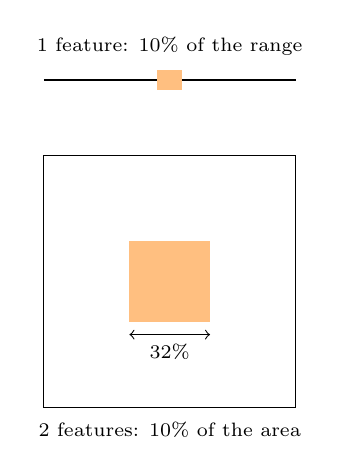
\begin{tikzpicture}[x=3.2cm, y=3.2cm]
                \draw[thick] (0, 1.3) -- (1, 1.3);
                \fill[orange!50] (0.45, 1.26) rectangle (0.55, 1.34);
                \node[font=\scriptsize, above] at (0.5, 1.36) {1 feature: 10\% of the range};
                \draw (0, 0) rectangle (1, 1);
                \fill[orange!50] (0.34, 0.34) rectangle (0.66, 0.66);
                \draw[<->] (0.34, 0.29) -- node[below, font=\scriptsize] {32\%} (0.66, 0.29);
                \node[font=\scriptsize, below] at (0.5, -0.02) {2 features: 10\% of the area};
            \end{tikzpicture}
        \end{column}
    \end{columns}
\end{frame}

\begin{frame}{Almost every point is extreme somewhere}
    \begin{columns}[T]
        \begin{column}{0.6\textwidth}
            \begin{itemize}
                \item Call a value extreme if it lies in the outer 5\% at either end of its feature's range (10\% of the values)
                \item A point is ordinary only if none of its values is extreme: for independent uniform features, $0.9^p$ of the points
                \item That is 81\% with two features, 35\% with ten and 0.5\% with fifty
                \item Nearly every point is then unusual in some feature, and predicting for it means extrapolating
            \end{itemize}
        \end{column}
        \begin{column}{0.38\textwidth}
            \centering
            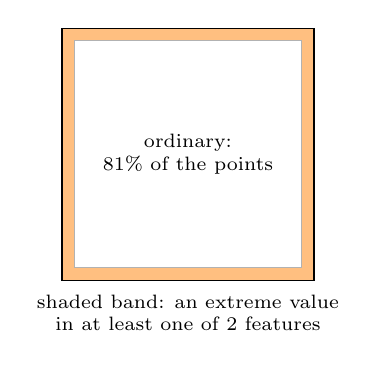
\begin{tikzpicture}[x=3.2cm, y=3.2cm]
                \fill[orange!50] (0, 0) rectangle (1, 1);
                \fill[white] (0.05, 0.05) rectangle (0.95, 0.95);
                \draw (0, 0) rectangle (1, 1);
                \draw[gray!60] (0.05, 0.05) rectangle (0.95, 0.95);
                \node[font=\scriptsize, align=center] at (0.5, 0.5) {ordinary:\\81\% of the points};
                \node[font=\scriptsize, below, align=center] at (0.5, -0.02) {shaded band: an extreme value\\in at least one of 2 features};
            \end{tikzpicture}
        \end{column}
    \end{columns}
\end{frame}

\begin{frame}{Everything is equally far away}
    \begin{itemize}
        \item The squared distance between two points adds up one term per feature
        \item A sum of many random terms varies little relative to its size (think of the average of many dice rolls)
        \item So as $p$ grows, all pairwise distances bunch together:
    \end{itemize}
    \centering
    \footnotesize
    \begin{tabular}{@{}r r r r r@{}}
        \toprule
        $p$ & Nearest pair & Mean & Farthest pair & Farthest / nearest \\
        \midrule
        2 & 0.001 & 0.525 & 1.341 & 1{,}496 \\
        10 & 0.300 & 1.258 & 2.339 & 7.78 \\
        100 & 2.909 & 4.084 & 5.130 & 1.76 \\
        1000 & 11.761 & 12.899 & 13.899 & 1.18 \\
        \bottomrule
    \end{tabular}

    {\scriptsize Pairwise distances between 500 uniform points in $[0, 1]^p$\par}
    \normalsize
    \raggedright
    \begin{itemize}
        \item When the nearest point is almost as far as the farthest, ``nearest'' tells us little
    \end{itemize}
\end{frame}

\begin{frame}{Bayes accuracy: the best any classifier can do}
    \begin{columns}[T]
        \begin{column}{0.6\textwidth}
            \begin{itemize}
                \item Classes overlap: some customers who default look just like customers who do not
                \item For customers who look alike, the best guess is the likelier class, and it is wrong for the rest: no model can avoid these mistakes
                \item The Bayes classifier (lecture 6) always picks the likelier class; its accuracy is a ceiling for every model
                \item Less overlap, higher ceiling: judge a model against it, not against 100\%
            \end{itemize}
        \end{column}
        \begin{column}{0.38\textwidth}
            \centering
            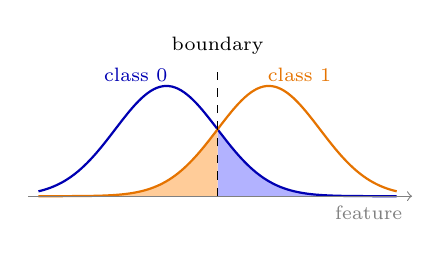
\begin{tikzpicture}[x=0.65cm, y=1.4cm, font=\scriptsize]
                \fill[blue!30] (1, 0) -- plot[domain=1:4.5, samples=40] (\x, {exp(-\x*\x/2)}) -- (4.5, 0) -- cycle;
                \fill[orange!40] (-2.5, 0) -- plot[domain=-2.5:1, samples=40] (\x, {exp(-(\x-2)*(\x-2)/2)}) -- (1, 0) -- cycle;
                \draw[thick, blue!70!black, domain=-2.5:4.5, samples=60, smooth] plot (\x, {exp(-\x*\x/2)});
                \draw[thick, orange!90!black, domain=-2.5:4.5, samples=60, smooth] plot (\x, {exp(-(\x-2)*(\x-2)/2)});
                \draw[->, gray] (-2.7, 0) -- (4.8, 0) node[below left] {feature};
                \draw[dashed] (1, 0) -- (1, 1.2) node[above] {boundary};
                \node[blue!70!black] at (-0.6, 1.1) {class 0};
                \node[orange!90!black] at (2.6, 1.1) {class 1};
            \end{tikzpicture}

            {\scriptsize Even the best boundary misclassifies the shaded tails}
        \end{column}
    \end{columns}
\end{frame}

\begin{frame}{Noise features drown the signal}
    \begin{columns}[T]
        \begin{column}{0.56\textwidth}
            \begin{itemize}
                \item Two classes differ in two features: no classifier can beat the Bayes accuracy of 0.856. We add $m$ pure-noise features with SD 1, so scaling is not the issue
                \item $k$-NN ($k = 15$) falls from 0.846 with no noise features to 0.811 with 20, 0.716 with 100 and 0.673 with 200
                \item Each noise feature adds a random term to every distance; together they outvote the two that matter
            \end{itemize}
        \end{column}
        \begin{column}{0.42\textwidth}
            \centering
            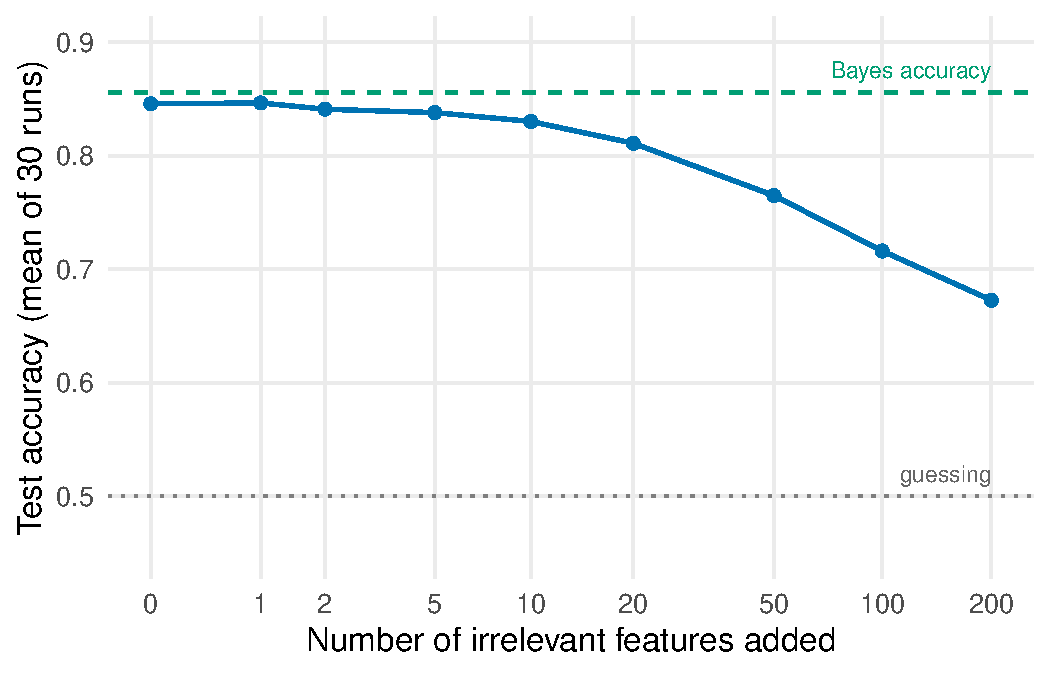
\includegraphics[width=\textwidth, height=0.75\textheight, keepaspectratio]{figures/fig_knn_noise_features.pdf}

            {\scriptsize 200 training and 1{,}000 test points; mean of 30 runs}
        \end{column}
    \end{columns}
\end{frame}


% \begin{frame}{Where the Bayes accuracy comes from}
%     \begin{itemize}
%         \item Class 0 is drawn around the mean $(0, 0)$ and class 1 around $(1.5, 1.5)$; the classes are equally likely, and in each class the two features have SD 1 and are uncorrelated
%         \item The Bayes classifier (lecture 6) then picks the class with the nearer mean; the boundary is the line halfway between them
%         \item The means are $\Delta = \sqrt{1.5^2 + 1.5^2} = 2.12$ apart, so each lies $\Delta / 2 = 1.06$ from the boundary
%         \item Along the line joining the means, a point's position is standard normal around its class mean, so it falls on the correct side with probability $\Phi(\Delta / 2) = \Phi(1.06) = 0.856$, where $\Phi$ is the standard normal CDF
%         \item The noise features are independent of the class, so the Bayes classifier ignores them: 0.856 is the ceiling for every $m$
%     \end{itemize}
% \end{frame}

\begin{frame}{More features, more ways to fit noise}
    \begin{columns}[T]
        \begin{column}{0.48\textwidth}
            \begin{itemize}
                \item OLS on $n = 100$ observations, where $y$ depends on only 5 of 99 features
                \item Training MSE keeps falling, to 0.083 at $p = 90$ and to 0 at $p = 99$
                \item Test MSE climbs from 1.06 at $p = 5$ to 2.04 at $p = 50$, 11.2 at $p = 90$ and 218 at $p = 99$
                \item Once $p + 1 > n$, $\mathbf{X}^\top\mathbf{X}$ is singular and OLS has no unique solution (lecture 3)
            \end{itemize}
        \end{column}
        \begin{column}{0.5\textwidth}
            \centering
            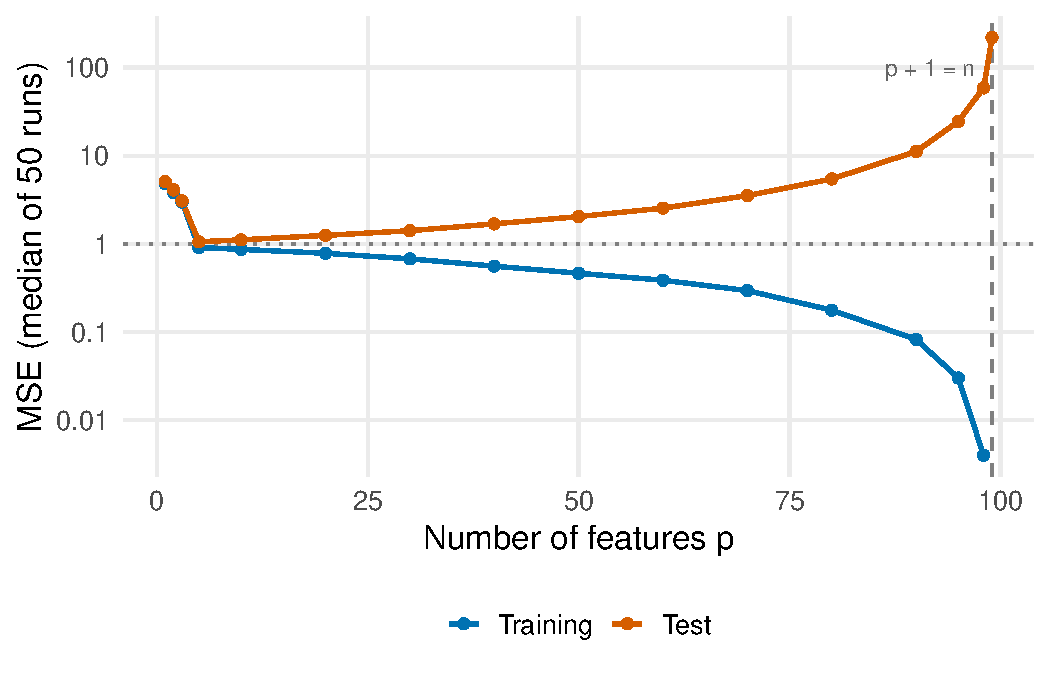
\includegraphics[width=\textwidth, height=0.6\textheight, keepaspectratio]{figures/fig_p_vs_n.pdf}

            {\scriptsize MSE: mean squared error on the fitting data (training) or new data (test); median over 50 data sets; dotted: best possible test MSE, 1}
        \end{column}
    \end{columns}
\end{frame}

\begin{frame}{Training error cannot choose $p$}
    \begin{itemize}
        \item Linear models suffer too: every feature is one more coefficient that can bend to the noise
        \item At $p = 99$ the model has 100 coefficients (with the intercept) for 100 observations and fits the training data exactly
        \item The extra features are pure noise, yet each one lowers the training error
        \item That is why training error cannot be used to choose $p$ (lecture 7)
    \end{itemize}
\end{frame}

\begin{frame}{What can we do?}
    \begin{itemize}
        \item Collect more data: rarely enough, since the data needed grows exponentially in $p$
        \item Regularize: ridge and lasso trade a little bias for much less variance (lecture 5)
        \item Select features: keep a subset of the original features (rest of this lecture)
        \item Extract features: build a few new features from all of them, e.g.\ PCA (lecture 12)
        \item Use domain knowledge to decide which features to collect and how to combine them
    \end{itemize}
\end{frame}

\begin{frame}{A caveat: real data are not uniform}
    \begin{itemize}
        \item The pictures above use independent, uniform features, which is the worst case
        \item Real features are correlated and the data concentrate near lower-dimensional structure (images, gene expression, survey items measuring the same trait)
        \item The intrinsic dimension of such data is much smaller than $p$
        \item This ``blessing of non-uniformity'' is why high-dimensional learning works at all, and why dimensionality reduction (lecture 12) succeeds
    \end{itemize}
\end{frame}


\section{Feature selection}

\begin{frame}{Selection vs. extraction}
    \begin{itemize}
        \item Feature selection keeps a subset of the original features
        \item Feature extraction builds new features from combinations of all of them (lecture 12)
        \item Reasons to select:
            \begin{itemize}
                \item Accuracy: fewer irrelevant features, lower variance
                \item Interpretability: a model with 5 named features can be explained
                \item Cost: features that are not used need not be measured, stored or computed
            \end{itemize}
        \item The methods fall into three families: filters, wrappers and embedded methods
    \end{itemize}
\end{frame}

\begin{frame}{Filter, wrapper, embedded}
    \centering
    \begin{tikzpicture}[
            box/.style={draw, rounded corners, minimum height=0.65cm, align=center, font=\scriptsize, fill=blue!8},
            lab/.style={font=\footnotesize\bfseries, anchor=east},
            >={Stealth[length=2mm]}, node distance=0.35cm
        ]
        \node[lab] at (-0.3, 0) {Filter};
        \node[box, anchor=west] (f1) at (0, 0) {All features};
        \node[box, right=of f1] (f2) {Score each feature\\ (no model)};
        \node[box, right=of f2] (f3) {Keep the\\ top features};
        \node[box, right=of f3, fill=orange!15] (f4) {Fit the model};
        \draw[->] (f1) -- (f2);
        \draw[->] (f2) -- (f3);
        \draw[->] (f3) -- (f4);

        \node[lab] at (-0.3, -1.7) {Wrapper};
        \node[box, anchor=west] (w1) at (0, -1.7) {All features};
        \node[box, right=of w1] (w2) {Propose a subset};
        \node[box, right=0.7cm of w2, fill=orange!15] (w3) {Fit the model,\\ estimate test error};
        \node[box, right=of w3] (w4) {Best subset};
        \draw[->] (w1) -- (w2);
        \draw[->] ([yshift=0.12cm]w2.east) -- ([yshift=0.12cm]w3.west);
        \draw[->] ([yshift=-0.12cm]w3.west) -- ([yshift=-0.12cm]w2.east);
        \draw[->] (w3) -- (w4);

        \node[lab] at (-0.3, -3.4) {Embedded};
        \node[box, anchor=west] (e1) at (0, -3.4) {All features};
        \node[box, right=of e1, fill=orange!15] (e2) {Fit a model that selects as it fits\\ (lasso, tree importance)};
        \node[box, right=of e2] (e3) {Subset and model};
        \draw[->] (e1) -- (e2);
        \draw[->] (e2) -- (e3);
    \end{tikzpicture}

    \svspace{0.6em}
    \footnotesize
    \begin{tabular}{@{}l l l l@{}}
        \toprule
        & Uses the model & Cost & Main risk \\
        \midrule
        Filter & no & low & ignores redundancy and interactions \\
        Wrapper & yes, as a black box & high & overfitting the search \\
        Embedded & yes, built in & moderate & tied to one model class \\
        \bottomrule
    \end{tabular}
\end{frame}

\begin{frame}{Filter: score features one at a time}
    \begin{itemize}
        \item A filter gives every feature a score on its own, before any model is fitted, and keeps the top scorers
        \item Typical scores: the correlation of the feature with a numeric response, or a test statistic that compares the feature's averages across classes
        \item Filters are fast, so they are the usual first pass when there are thousands of features
        \item The price is that each feature is judged alone. Redundant features, which carry the same information, all score high and all get kept
        \item Features that help only in combination (an interaction) can each score near zero and both get thrown away: think of a class that is 1 exactly when two features have the same sign
    \end{itemize}
\end{frame}

\begin{frame}{Filter: redundant and constant features}
    \begin{columns}[T]
        \begin{column}{0.56\textwidth}
                        \begin{itemize}
                \item The Credit data (ISLP package): balances of 400 card holders, 11 predictor columns
                \item Limit and Rating are nearly the same variable ($r = 0.997$), the only pair above 0.9 (collinearity, lecture 4)
                \item Keep one; it hardly matters which, since both correlate about equally with Balance (0.862 and 0.864)
                \item Also drop constant or nearly constant features (variance threshold)
            \end{itemize}
        \end{column}
        \begin{column}{0.42\textwidth}
            \centering
            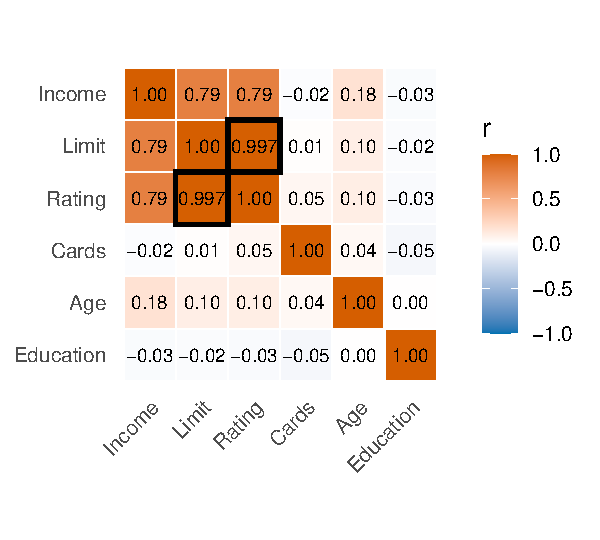
\includegraphics[width=\textwidth, height=0.75\textheight, keepaspectratio]{figures/fig_filter_corr.pdf}
        \end{column}
    \end{columns}
\end{frame}


% \begin{frame}{Filter: univariate scores}
%     \centering
%     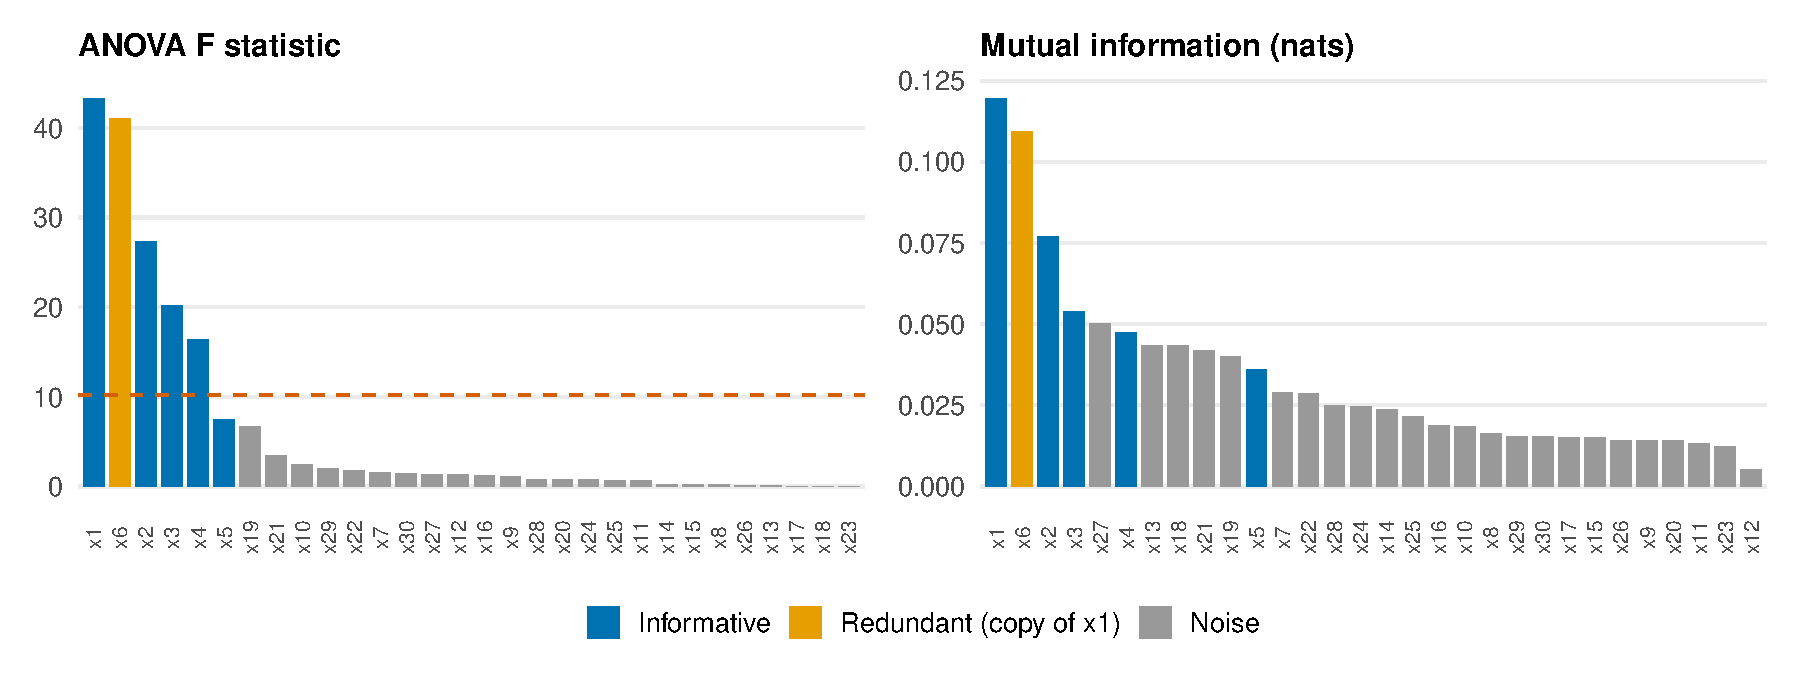
\includegraphics[width=\textwidth, height=0.44\textheight, keepaspectratio]{figures/fig_filter_scores.pdf}
%     \raggedright
%     \footnotesize
%     \begin{itemize}
%         \item Simulation with $n = 200$ and binary $y$: $x_1, \dots, x_5$ are informative, $x_6$ is a noisy copy of $x_1$ ($r = 0.954$), and $x_7, \dots, x_{30}$ are noise
%         \item The $F$ statistic ($F = t^2$ for two classes) compares class means; use the correlation for a numeric $y$, and $\chi^2$ for categorical features
%         \item Both scores rank $x_6$ second: a filter judges features one at a time, so it cannot see that $x_6$ repeats $x_1$
%     \end{itemize}
% \end{frame}


% \begin{frame}{Mutual information}
%     \begin{itemize}
%         \item Mutual information $I(X; Y)$ measures how much knowing $X$ reduces uncertainty about $Y$; it is 0 only under independence and also picks up nonlinear dependence
%         \item Defined as $\displaystyle I(X; Y) = \sum_{x, y} p(x, y) \log \frac{p(x, y)}{p(x)\,p(y)}$, measured in nats with the natural logarithm
%         \item Here each feature is cut into 10 bins at its deciles, and the probabilities are estimated by relative frequencies; scikit-learn's \texttt{mutual\_info\_classif} uses a nearest-neighbor estimator instead
%         \item Mutual information is noisier than the $F$ statistic: the largest value among the 24 noise features (0.05) exceeds that of the informative $x_5$ (0.036)
%     \end{itemize}
% \end{frame}


% \begin{frame}{Filter pitfall: multiple testing}
%     \begin{itemize}
%         \item Keeping every feature with $p$-value below 0.05 keeps about 5\% of the noise features
%         \item In the simulation, 1 of the 24 noise features has $p < 0.05$, close to the 1.2 expected by chance
%         \item With 5{,}000 noise features, about 250 would get through
%         \item The Bonferroni threshold $0.05/30 = 0.00167$ ($F > 10.16$, the dashed line on the previous plot) keeps $x_1, \dots, x_4$ and $x_6$ and no noise features, but it misses $x_5$ ($F = 7.4$)
%         \item A score threshold controls false discoveries, not predictive accuracy, so choose the number of features by cross-validation
%     \end{itemize}
% \end{frame}


% \begin{frame}{Filter pitfall: interactions}
%     \centering
%     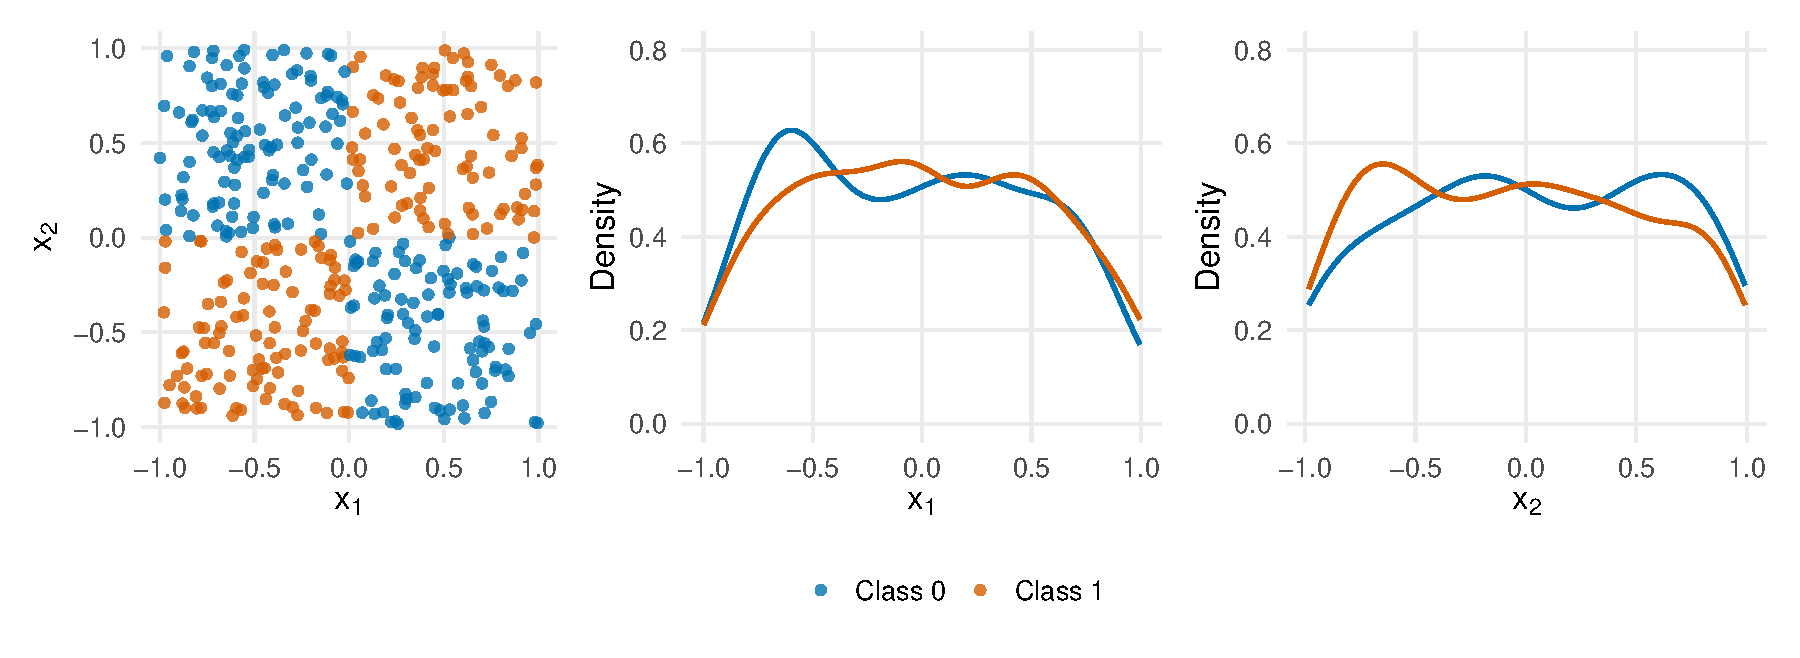
\includegraphics[width=\textwidth, height=0.4\textheight, keepaspectratio]{figures/fig_xor.pdf}
%     \raggedright
%     \begin{itemize}
%         \item In this ``XOR'' data set of 400 uniform points, the class is 1 when $x_1$ and $x_2$ have the same sign
%         \item On its own, each feature looks useless: the $t$-test $p$-values are 0.40 and 0.22, and the class densities overlap
%         \item Yet $k$-NN reaches 0.946 test accuracy with both features, against 0.506 with $x_1$ alone
%         \item A univariate filter would throw both features away
%     \end{itemize}
% \end{frame}

\begin{frame}{Wrapper: best subset selection}
    \begin{enumerate}
        \item For each size $k = 1, \dots, p$, fit all $\binom{p}{k}$ models with $k$ features and keep the one with the smallest training RSS (residual sum of squares)
        \item Choose among the $p$ winners with an estimate of test error: cross-validation, or $C_p$/AIC, BIC and adjusted $R^2$, which penalize large models
    \end{enumerate}
    \svspace{0.5em}
    \begin{itemize}
        \item Training RSS always prefers the largest model, so it can only compare models of the same size
        \item That is $2^p$ models in all: 2{,}048 for Credit's 11 columns, about $10^6$ for $p = 20$ and about $1.1 \times 10^{12}$ for $p = 40$
        \item This is feasible up to $p \approx 30$--$40$ for linear regression, and searching so many models also overfits the selection
    \end{itemize}
\end{frame}

\begin{frame}{Wrapper: forward and backward selection}
    \begin{columns}[T]
        \begin{column}{0.6\textwidth}
                        \begin{itemize}
                \item Forward starts empty and keeps adding the most helpful feature: $1 + p(p + 1)/2$ fits, 67 for Credit
                \item Backward starts full and drops the least useful one; it needs $n > p$
                \item Both are greedy (no step is ever undone). At size 4, best subset picks Income, Limit, Cards, Student; forward, stuck with Rating, ends with Income, Limit, Rating, Student
                \item BIC chooses 4 features for best subset and backward, 5 for forward
            \end{itemize}
        \end{column}
        \begin{column}{0.38\textwidth}
            \centering
            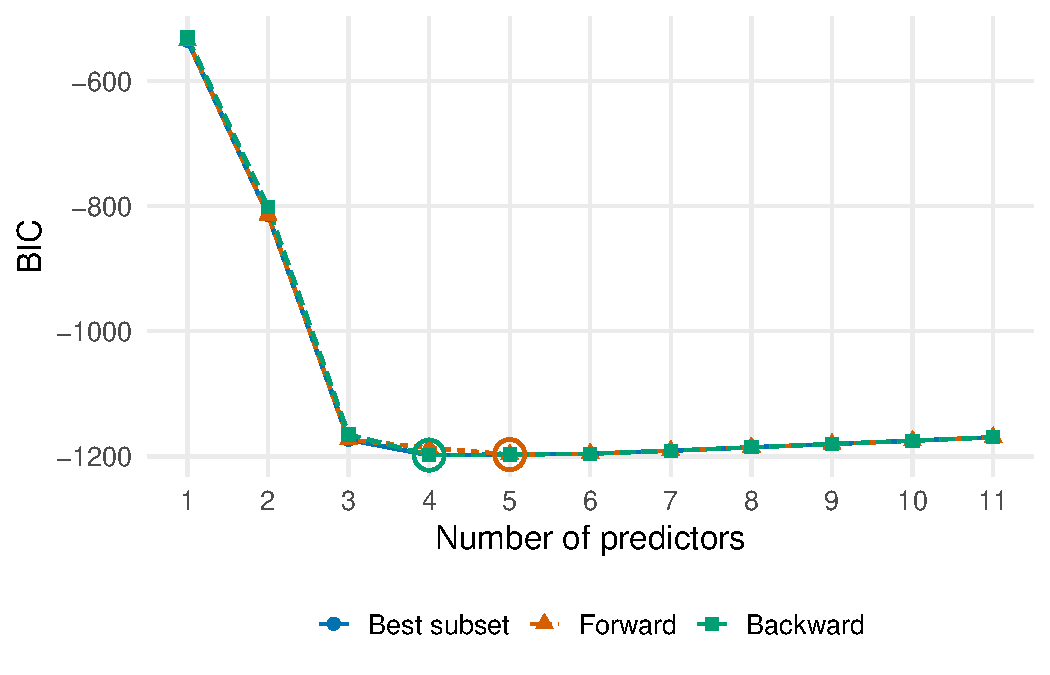
\includegraphics[width=\textwidth, height=0.75\textheight, keepaspectratio]{figures/fig_subset_selection.pdf}

            {\scriptsize Credit: BIC by size; circles mark the minima}
        \end{column}
    \end{columns}
\end{frame}

\begin{frame}{Subset selection: details}
    \begin{itemize}
        \item BIC scores fit plus a charge per feature; for a linear model with $d$ features it is, up to a constant, $n \log(\mathrm{RSS}/n) + d \log n$, and lower is better
        \item Its penalty of $\log n$ per feature is larger than AIC's $2$ once $n > 7$, so BIC prefers smaller models (ISLP Section 6.1)
        \item Backward selection disagrees with best subset at sizes 1 to 3, because it starts with Limit and Rating together and drops Rating before Limit
        \item Hybrid (stepwise) methods allow a feature to be removed after it has been added
    \end{itemize}
\end{frame}

\begin{frame}{Wrapper: recursive feature elimination}
    \begin{columns}[T]
        \begin{column}{0.56\textwidth}
                        \begin{itemize}
                \item Fit the model on all features, drop the weakest (smallest $|\hat{\beta}_j|$ on standardized features, or lowest importance), refit, and repeat
                \item Here: logistic regression on the 30-feature simulation, with RFE rerun inside each of 10 CV folds
                \item CV accuracy is 0.79 with all 30 features and peaks at 0.82 with 5
                \item On all the data, RFE ranks $x_1, \dots, x_5$ first: exactly the informative features
            \end{itemize}
        \end{column}
        \begin{column}{0.42\textwidth}
            \centering
            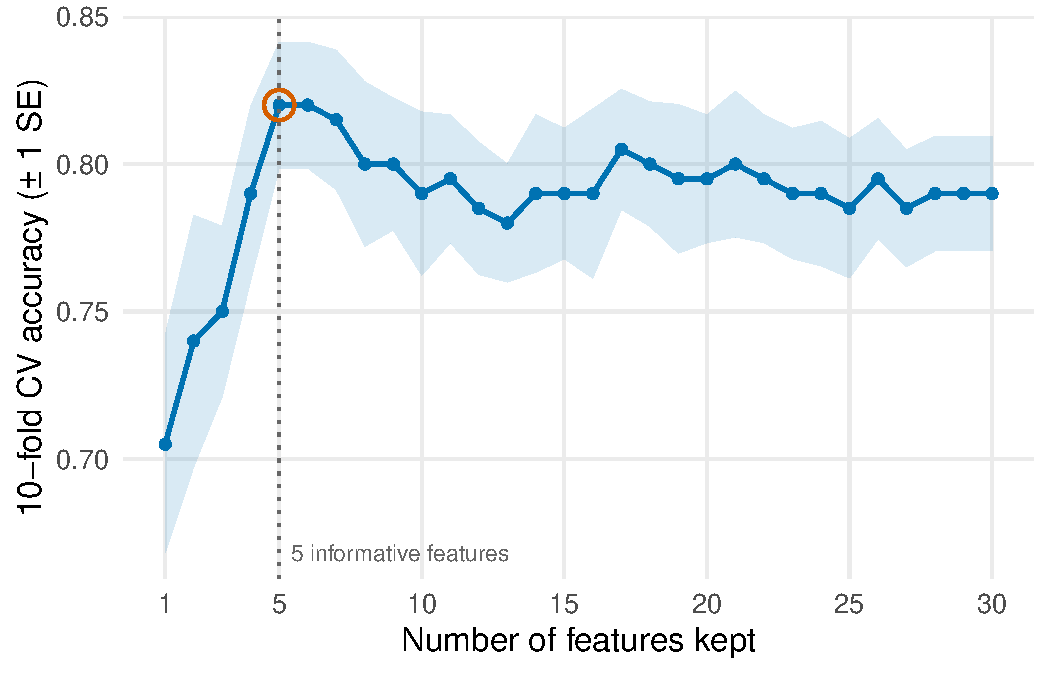
\includegraphics[width=\textwidth, height=0.6\textheight, keepaspectratio]{figures/fig_rfe.pdf}

            {\scriptsize Simulated data: 200 observations, 30 features; $y$ depends on $x_1, \dots, x_5$, $x_6$ is a noisy copy of $x_1$, the rest is noise}
        \end{column}
    \end{columns}
\end{frame}

\begin{frame}{Ridge and lasso: a price on large coefficients}
    \begin{itemize}
        \item Ordinary least squares picks the coefficients that fit the training data best, even if that takes large, unstable coefficients that chase noise
        \item Ridge and lasso minimize misfit plus a price for large coefficients (the intercept is not charged):
        \[
            \begin{aligned}
                \text{ridge:} \quad & \frac{1}{2n}\lVert \mathbf{y} - \mathbf{X}\boldsymbol{\beta} \rVert^2 + \frac{\lambda}{2} \sum_{j=1}^{p} \beta_j^2 \\
                \text{lasso:} \quad & \frac{1}{2n}\lVert \mathbf{y} - \mathbf{X}\boldsymbol{\beta} \rVert^2 + \lambda \sum_{j=1}^{p} |\beta_j|
            \end{aligned}
        \]
        \item $\lambda$ is the dial: $\lambda = 0$ gives ordinary least squares, and the larger $\lambda$, the harder all coefficients are pulled toward 0
    \end{itemize}
\end{frame}

\begin{frame}{How ridge and lasso shrink a coefficient}
    \begin{columns}[T]
        \begin{column}{0.54\textwidth}
            \begin{itemize}
                \item Ridge pulls with a strength proportional to the coefficient: all coefficients shrink smoothly and none reaches exactly 0
                \item The lasso pulls with a constant strength: a coefficient with weak evidence ends at exactly 0 and its feature drops out, so the lasso selects features
            \end{itemize}
        \end{column}
        \begin{column}{0.44\textwidth}
            \centering
            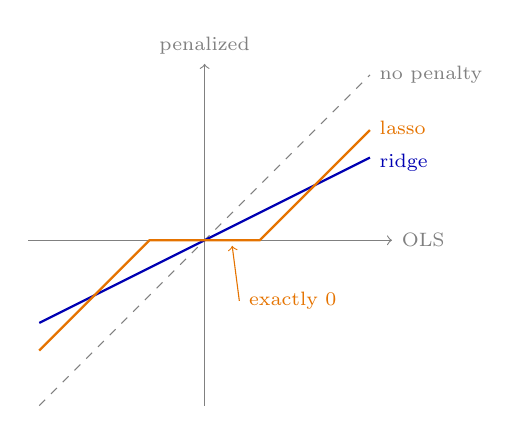
\begin{tikzpicture}[x=0.7cm, y=0.7cm, font=\scriptsize]
                \draw[->, gray] (-3.2, 0) -- (3.4, 0) node[right] {OLS};
                \draw[->, gray] (0, -3.0) -- (0, 3.2) node[above] {penalized};
                \draw[dashed, gray] (-3, -3) -- (3, 3);
                \draw[thick, blue!70!black] (-3, -1.5) -- (3, 1.5);
                \draw[thick, orange!90!black] (-3, -2) -- (-1, 0) -- (1, 0) -- (3, 2);
                \node[gray, anchor=west] at (3, 3) {no penalty};
                \node[orange!90!black, anchor=west] at (3, 2.05) {lasso};
                \node[blue!70!black, anchor=west] at (3, 1.4) {ridge};
                \node[orange!90!black] (z) at (1.6, -1.1) {exactly 0};
                \draw[->, orange!90!black] (z.west) -- (0.5, -0.1);
            \end{tikzpicture}

            {\scriptsize Coefficient with and without the penalty (uncorrelated, standardized features)}
        \end{column}
    \end{columns}
\end{frame}

\begin{frame}{Embedded: the lasso}
    \begin{itemize}
        \item Minimize $\frac{1}{2n}\lVert \mathbf{y} - \mathbf{X}\boldsymbol{\beta} \rVert^2 + \lambda \sum_j |\beta_j|$: the $L_1$ penalty sets some coefficients exactly to 0; ridge only shrinks them, and at the same $\lambda$ sets none exactly to 0
    \end{itemize}
    \centering
    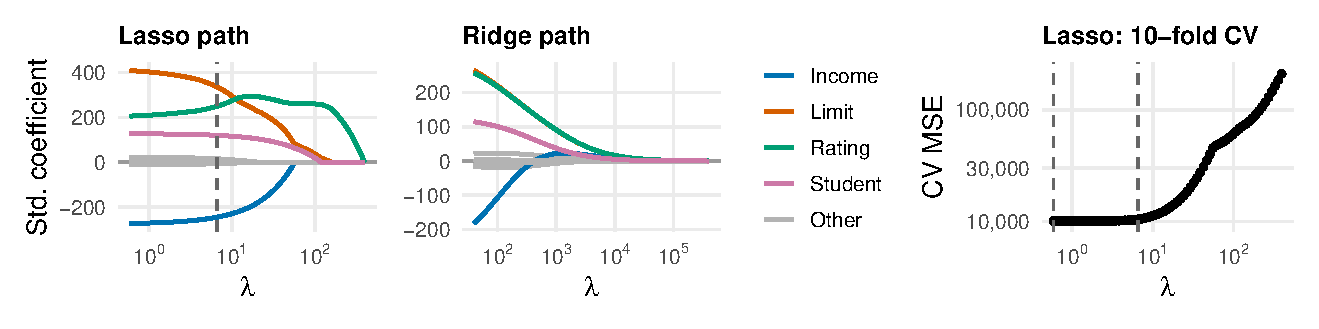
\includegraphics[width=\textwidth, height=0.4\textheight, keepaspectratio]{figures/fig_lasso_path.pdf}
    \raggedright
    \footnotesize
    \begin{itemize}
        \item On Credit, Rating enters the path first, followed by Limit, Student and Income
        \item With 10-fold CV, $\lambda_{\min}$ keeps all 11 columns (CV MSE 10{,}067), while $\lambda_{1\mathrm{SE}}$, the largest $\lambda$ within one standard error of the minimum, keeps 6: Income, Limit, Rating, Cards, Age, Student (CV MSE 10{,}455)
    \end{itemize}
\end{frame}

\begin{frame}{Reading the lasso and ridge paths}
    \begin{itemize}
        \item Each line in the path plots on the previous slide is one coefficient; moving right, $\lambda$ grows and the lines shrink toward 0
        \item In the lasso panel they hit exactly 0 one after another, so features drop out one by one; in the ridge panel they only approach 0
        \item The right panel shows the CV error for each $\lambda$: $\lambda_{\min}$ has the lowest error, $\lambda_{1\mathrm{SE}}$ is the largest $\lambda$ whose error is within one standard error of the lowest
        \item $\lambda_{1\mathrm{SE}}$ is the simplest model that cross-validation cannot tell apart from the best, a common choice when a small, interpretable model is the goal
    \end{itemize}
\end{frame}

\begin{frame}{Embedded: importance from tree ensembles}
    \begin{columns}[T]
        \begin{column}{0.58\textwidth}
            \begin{itemize}
                \item Impurity importance adds up the Gini decrease (how much a split purifies a node) from every split on a feature, on the training data
                \item It favors features with many split points: a continuous noise feature ranks second (60.1), above an informative binary one (54.7)
                \item Permutation importance is the drop in out-of-bag accuracy (on observations a tree did not see) when a feature is shuffled; noise scores about 0
            \end{itemize}
        \end{column}
        \begin{column}{0.4\textwidth}
            \centering
            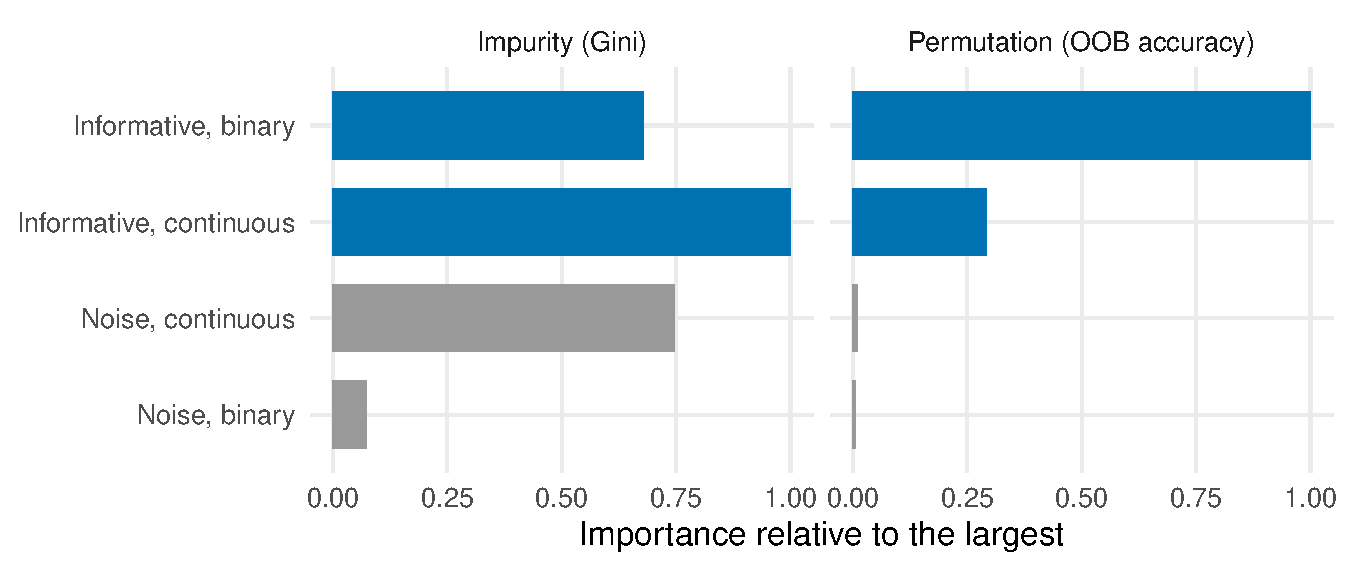
\includegraphics[width=\textwidth, height=0.75\textheight, keepaspectratio]{figures/fig_importance.pdf}

            {\scriptsize Random forest, 500 trees; mean over 20 data sets of 500 observations}
        \end{column}
    \end{columns}
\end{frame}

\begin{frame}{Correlated features in the lasso and in importance}
    \begin{itemize}
        \item The lasso path plots show standardized coefficients (coefficient times the SD of the feature), so that features are comparable
        \item The lasso has no preference between strongly correlated features: along the path it switches between Limit and Rating, and a small change in the data can change which one it keeps
        \item Permutation importances in the simulation: 0.129 for the informative binary feature, 0.038 for the informative continuous one, 0.0013 and 0.0007 for the two noise features
        \item When features are correlated, shuffling one of them leaves its partner in place, so permutation importance spreads the credit between them and can understate both
    \end{itemize}
\end{frame}


% \begin{frame}{Select inside cross-validation}
%     \begin{columns}[T]
%         \begin{column}{0.5\textwidth}
%             \begin{itemize}
%                 \item With $n = 50$, 5{,}000 noise features and random labels, no classifier can beat 0.5
%                 \item Keep the 20 features with the largest $|t|$, then run 5-NN with 5-fold CV; repeat 200 times
%                 \item Selecting on all 50 first gives a mean CV accuracy of 0.941, never below 0.8
%                 \item Selecting inside each training fold gives 0.472. Selection is part of fitting, so it belongs in the pipeline
%             \end{itemize}
%         \end{column}
%         \begin{column}{0.48\textwidth}
%             \centering
%             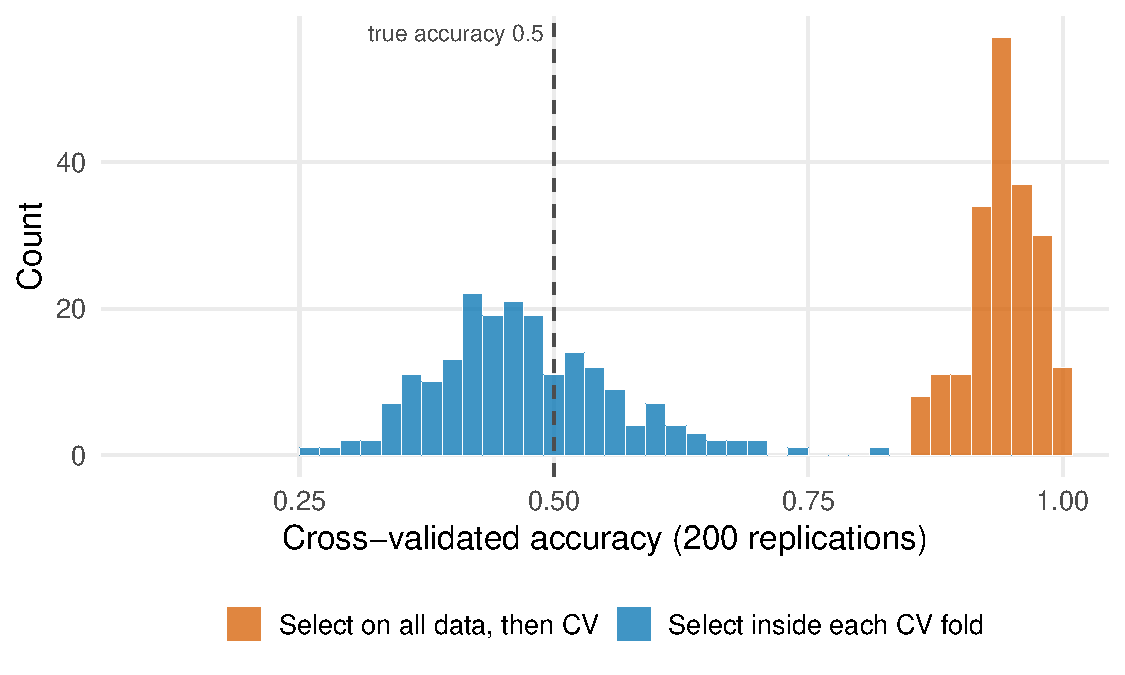
\includegraphics[width=\textwidth, height=0.75\textheight, keepaspectratio]{figures/fig_selection_leakage.pdf}
%         \end{column}
%     \end{columns}
% \end{frame}


% \begin{frame}{Why selecting first goes wrong}
%     \begin{itemize}
%         \item Selecting on all the data picks the 20 features that happen to separate the labels of all 50 observations, the held-out ones included, so every held-out fold has already been seen (\emph{The Elements of Statistical Learning}, Section 7.10.2)
%         \item The correct estimate, 0.472, is slightly below 0.5, a known effect of cross-validation with random labels
%         \item Holding out a fold removes more of one class than the other, so the training folds are tilted towards the class that is under-represented in the held-out fold
%     \end{itemize}
% \end{frame}

\begin{frame}{Choosing a method}
    \centering
    \footnotesize
    \begin{tabular}{@{}l l@{}}
        \toprule
        Situation & Start with \\
        \midrule
        Thousands of features, first pass & filter: variance, correlation, univariate scores \\
        Linear model, interpretable result & lasso with $\lambda$ chosen by CV \\
        Small $p$, cheap model fits & best subset or stepwise, with CV or BIC \\
        Any model, moderate $p$ & RFE inside CV \\
        Tree ensembles & permutation importance \\
        \bottomrule
    \end{tabular}

    \svspace{0.8em}
    \raggedright
    \begin{itemize}
        \item Whatever the method, choose the number of features by cross-validation, with selection inside the folds
    \end{itemize}
\end{frame}


\section{Summary}

\begin{frame}{Scaling and selection in Python}
    \centering
    \scriptsize
    \begin{tabular}{@{}l l@{}}
        \toprule
        Task & Python (\texttt{sklearn}) \\
        \midrule
        Scalers & \texttt{preprocessing.StandardScaler}, \texttt{MinMaxScaler}, \texttt{RobustScaler} \\
        Row normalization & \texttt{preprocessing.Normalizer} \\
        Skewed features & \texttt{preprocessing.PowerTransformer} (Box-Cox, Yeo-Johnson) \\
        Pipelines & \texttt{pipeline.make\_pipeline}, \texttt{compose.ColumnTransformer} \\
        Variance filter & \texttt{feature\_selection.VarianceThreshold} \\
        Univariate scores & \texttt{feature\_selection.SelectKBest(f\_classif)}, \texttt{mutual\_info\_classif} \\
        Forward, backward & \texttt{feature\_selection.SequentialFeatureSelector} \\
        RFE & \texttt{feature\_selection.RFE}, \texttt{RFECV} \\
        Lasso & \texttt{linear\_model.LassoCV}; \texttt{LogisticRegression(penalty="l1")} \\
        Permutation importance & \texttt{inspection.permutation\_importance} \\
        \bottomrule
    \end{tabular}

    \svspace{0.5em}
    Worked examples: the ISLP Python lab, Section 6.5
\end{frame}

\begin{frame}{Summary}
    \begin{itemize}
        \item Scale features for distance-based methods, kernels, PCA, penalized models and gradient descent; fit the scaler on training data only, inside a pipeline
        \item In high dimensions data are sparse, distances concentrate and noise features swamp local methods
        \item Filters are cheap but blind to redundancy and interactions; wrappers search subsets with a model; the lasso and tree ensembles select while fitting
        \item Feature selection is part of the model: do it inside cross-validation
        \item Reading: ISLP 6.1, 6.2 and 6.4; ESL 2.5 and 7.10.2
        \item Next lecture: instead of selecting features, we build new ones with the SVD and PCA
    \end{itemize}
\end{frame}